\section{Implementation}
Since the system of equations (\ref{eqn:full_model}) is highly nonlinear, its solution requires a scheme such as Newton's method. In chapter \ref{chap:large_fem} a finite element scheme using Newton's method for the solution of the poroelastic equations valid in large deformations (\ref{eqn:simple_mixture_model}) has already been presented. In this chapter we adopt the same finite element scheme as presented in chapter \ref{chap:large_fem} for solving the poroelastic equations and expand the linear system (discretized linearization) to include additional matrices required for solving the fluid network and its coupling to the poroelastic medium (equations (\ref{eqn:mixture_mass_reform_full},\ref{eqn:tree_flow},\ref{eqn:tree_mass},\ref{eqn:pressure_coupling})). This results in a monolithic coupling scheme that ensures good convergence even for problems with strong coupling interactions between the poroelastic medium and the fluid network (see section \ref{sec:constriction}). For details on how the stiffness matrix $\boldsymbol{K}$ (discretized linearization of the full lung model (\ref{eqn:full_model})), and the residual vector $\boldsymbol{R}$ are built, see section \ref{sec:fem_appendix}. To solve the nonlinear poroelastic problem using Newton's method at a particular time step, we perform the the steps already described in algorithm \ref{algo:newton}. We set the relative tolerance to be $\mbox{TOL}=10^{-4}$. For the subsequent numerical results shown in section \ref{sec:numerical_results}, a maximum of $5$ Newton iterations were required to solve each time step.






\subsection{Discrete coupling of the fluid network to the poroelastic model}
\label{sec:coupling_appendix}
If we discretize the space using triangles and employ a piecewise constant pressure approximation (one node at the center of each element), the resulting coupling for the simple 2D example (Figure \ref{fig:domains_cont}) is shown in Figure \ref{fig:coupling_disc1}. Once we refine the mesh (Figure \ref{fig:coupling_disc2}), the discretized division of subdomains tends to the subdivision of the original problem (Figure \ref{fig:domains_cont}).
%
The $i$th discretized subdomain $\Omega_{t}^{i}$ is defined as the set of elememts, $E$, closest to the position of the $i$th inlet, denoted by $\mbox{pos}(P_{di})$. 
\begin{equation}
\Omega_{t}^{i} := \left\lbrace E \in \Omega_{t} : ||\mbox{pos}(P_{di}) - \mbox{cent}(E) || <  ||\mbox{pos}(P_{dk}) - \mbox{cent}(E) ||, \;k=1,2...,N \,, k \neq i \right\rbrace,
 \label{discrete_subdomain_definition}
\end{equation} 
where $ \mbox{cent}(E)$ denotes the centroid of an element.
%This highlights that the numerical approximation is not mesh dependent, provided a fine enough mesh discretisation is used.
\begin{figure}[h]
\centering
\subfloat[]{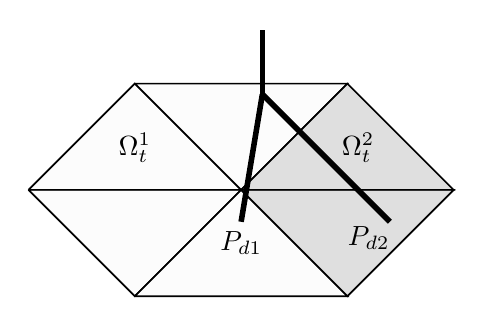
\begin{tikzpicture}[scale=1.35]
  %Coarse discretisation
  \draw[semithick,fill=black!2,fill opacity=0.5] 
    (0,1) to (1,2) to  (2,1) to (0,1) ;
  \draw[semithick,fill=black!2,fill opacity=0.5] 
    (0,1) to (1,0) to  (2,1) to (0,1) ; 
  \draw[semithick,fill=black!2,fill opacity=0.5] 
    (1,2) to (2,1) to  (3,2) to (1,2) ;
   \draw[semithick,fill=black!2,fill opacity=0.5] 
    (1,0) to (2,1) to  (3,0) to (1,0) ;
    \draw[semithick,fill=black!25,fill opacity=0.5] 
    (2,1) to (3,2) to  (4,1) to (2,1) ;
  \draw[semithick,fill=black!25,fill opacity=0.5] 
    (2,1) to (3,0) to  (4,1) to (2,1) ;

   %TREE
  \draw[line width=2pt] (2.2,1.9) -- (2.2,2.5);
  \draw[line width=2pt] (3.4,0.7) -- (2.2,1.9);
  \draw[line width=2pt] (2,0.7) -- (2.2,1.9);
    		     	
	%Labelling
	\draw (3.2,0.55) node {$P_{d2}$};
	\draw (3.1,1.4) node {  $\Omega_{t}^{2}$};
	\draw (2,0.5) node {$P_{d1}$};
	\draw (1,1.4) node {  $\Omega_{t}^{1}$};	
\end{tikzpicture}
\label{fig:coupling_disc1}
}
\subfloat[]{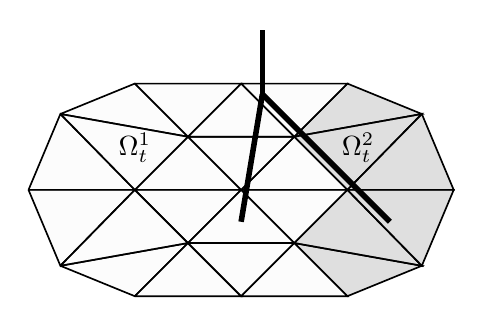
\begin{tikzpicture}[scale=1.35]

  %Top left tri
  \draw[semithick,fill=black!2,fill opacity=0.5] 
    (0,1) to (0.3,1.7141) to  (1,1) to (0,1) ;
   \draw[semithick,fill=black!2,fill opacity=0.5] 
    (1,1) to (1.5,1.5) to  (2,1) to (1,1) ;
  \draw[semithick,fill=black!2,fill opacity=0.5] 
    (0.3,1.7141) to (1,2) to  (1.5,1.5) to (0.3,1.7141) ;
    \draw[semithick,fill=black!2,fill opacity=0.5] 
    (0.3,1.7141) to (1.5,1.5) to  (1,1) to (0.3,1.7141) ;
    
   %Top right tri
   \draw[semithick,fill=black!25,fill opacity=0.5] 
    (2.5,1.5) to (3,2) to  (3.7,1.7141) to (2.5,1.5) ;
       \draw[semithick,fill=black!25,fill opacity=0.5] 
    (2.5,1.5) to (3.7,1.7141) to  (3,1) to (2.5,1.5) ;
  \draw[semithick,fill=black!2,fill opacity=0.5] 
    (2,1) to (2.5,1.5) to  (3,1) to (2,1) ;
   \draw[semithick,fill=black!25,fill opacity=0.5] 
   (3,1) to (3.7,1.7141) to  (4,1) to (3,1) ;

   %Bottom left
   \draw[semithick,fill=black!2,fill opacity=0.5] 
    (0,1) to (0.3,0.2859) to  (1,1) to (0,1) ;
   \draw[semithick,fill=black!2,fill opacity=0.5] 
    (1,1) to (1.5,0.5) to  (2,1) to (1,1) ;
  \draw[semithick,fill=black!2,fill opacity=0.5] 
    (0.3,0.2859) to (1,0) to  (1.5,0.5) to (0.3,0.2859) ;
    \draw[semithick,fill=black!2,fill opacity=0.5] 
    (0.3,0.2859) to (1.5,0.5) to  (1,1) to (0.3,0.2859) ;

 
    %Bottom right
  \draw[semithick,fill=black!25,fill opacity=0.5] 
    (2.5,0.5) to (3,0) to  (3.7,0.2859) to (2.5,0.5) ;
       \draw[semithick,fill=black!25,fill opacity=0.5] 
    (2.5,0.5) to (3.7,0.2859) to  (3,1) to (2.5,0.5) ;
  \draw[semithick,fill=black!2,fill opacity=0.5] 
    (2,1) to (2.5,0.5) to  (3,1) to (2,1) ;
   \draw[semithick,fill=black!25,fill opacity=0.5] 
   (3,1) to (3.7,0.2859) to  (4,1) to (3,1) ;
 
  %Bottom middle - to do
  \draw[semithick,fill=black!2,fill opacity=0.5] 
    (1.5,0.5) to (2,1) to  (2.5,0.5) to (1.5,0.5) ;
  \draw[semithick,fill=black!2,fill opacity=0.5] 
    (1,0) to (1.5,0.5) to  (2,0) to (1,0) ;
  \draw[semithick,fill=black!2,fill opacity=0.5] 
    (2,0) to (2.5,0.5) to  (3,0) to (2,0) ;
  \draw[semithick,fill=black!2,fill opacity=0.5] 
    (1.5,0.5) to (2,0) to  (2.5,0.5) to (1.5,0.5) ;
    
  %Top Middle
  \draw[semithick,fill=black!2,fill opacity=0.5] 
    (1.5,1.5) to (2,1) to  (2.5,1.5) to (1.5,1.5) ;
  \draw[semithick,fill=black!2,fill opacity=0.5] 
    (1,2) to (1.5,1.5) to  (2,2) to (1,2) ;
  \draw[semithick,fill=black!2,fill opacity=0.5] 
    (2,2) to (2.5,1.5) to  (3,2) to (2,2) ;
  \draw[semithick,fill=black!2,fill opacity=0.5] 
    (1.5,1.5) to (2,2) to  (2.5,1.5) to (1.5,1.5) ; 
   %TREE
   \draw[line width=2pt] (2.2,1.9) -- (2.2,2.5);
   \draw[line width=2pt] (3.4,0.7) -- (2.2,1.9);
   \draw[line width=2pt] (2,0.7) -- (2.2,1.9);	
	%Labelling
	%\draw (3.2,0.55) node {$P_{d2}$};
	\draw (3.1,1.4) node {  $\Omega_{t}^{2}$};
	%\draw (2,0.5) node {$P_{d1}$};
	\draw (1,1.4) node {  $\Omega_{t}^{1}$};	
\end{tikzpicture}
\label{fig:coupling_disc2}
}
\caption{(a) Coupling between the discretized domain and the fluid network using a piecewise constant pressure approximation for the example shown in Figure \ref{fig:domains_cont}. (b) Coupling between the discretized domain and the fluid network after mesh refinement.} 
\label{fig:coupling}
\end{figure}



\subsection{Finite element matrices}
\label{sec:fem_appendix}
For the fully-coupled large deformation poroelastic fluid network model we need to solve the linear system $\boldsymbol{K}(\mathfrak{u}_{i}^{n}) \change \mathfrak{u}_{i+1}^{n} = - \boldsymbol{R}(\mathfrak{u}_{i}^{n},\mathfrak{u}^{n-1})$ at each Newton iteration. This can be expanded as
%
 \begin{equation*}
 \begin{bmatrix}
   \mathbf{K}^{e} & 0 & \mathbf{B}^{T} & 0  & 0 & 0 & 0&  0\\
  0 & \mathbf{M} & \mathbf{B}^{T} & \mathbf{L}^{T}  & 0& 0 & 0&  0\\
 -  \mathbf{B} & -\Delta t \mathbf{B} & \mathbf{J} & 0 & 0 & 0&  0 & -\Delta t \mathbf{G}^{T} \\
 0 & \mathbf{L} & 0 & 0 & 0 &  0 & 0 &  0\\
 0 & 0 & 0& 0 &  \mathbf{T}_{11}   &   \cdots & \cdots& \mathbf{T}_{14} \\
 0 & 0 & 0& 0 & \vdots\  & &     & \vdots\\
0 & 0 & 0& 0 & \mathbf{T}_{31}  & \cdots &\cdots & \mathbf{T}_{34}\\
 0 & 0 & \mathbf{G} & 0 & 0 &  -\mathbf{X}  &  0&  0 \\
 \end{bmatrix}
 \begin{bmatrix}
  \change\mathbf{u}^{n} \\
  \change\mathbf{z}^{n} \\
 \change\mathbf{p}^{n}  \\
\change\mathbf\Lambda^{n}  \\
\change\mathbf{P}^{n}  \\
\change\mathbf{P}^{n}_{d}  \\
\change\mathbf{Q}^{n}  \\
\change\mathbf{Q}_{d}^{n}  \\
 \end{bmatrix}=-
 \begin{bmatrix}
  \boldsymbol{r}_{1} \\
  \boldsymbol{r}_{2} \\
 \boldsymbol{r}_{3} -\Delta t \mathbf{G}^{T} \mathbf{Q}_{d}^{n} \\
0 \\
0 \\
0 \\
0 \\
\mathbf{G} \mathbf{p}^{n} - \mathbf{X} \mathbf{P}^{n}_{d}
 \end{bmatrix},
 \end{equation*}
 where we have defined the following matrices and vectors:
 \begin{equation*}
  \boldsymbol{K}^{e}=[\boldsymbol{a}_{kl}], \;\; \boldsymbol{k}^{e}_{kl}=\int_{{\Omega_{t} }} \boldsymbol{E}^{T}_{k}\boldsymbol{D}(\boldsymbol{u}^{n}_{i})\boldsymbol{E}_{l}+  (\nabla \boldsymbol{\phi}_{k})^{T}\boldsymbol{\sigma}_{e}(\boldsymbol{u}^{n}_{i})\nabla \boldsymbol{\phi}_{l}  \; dv,
 \end{equation*}
 \begin{equation*}
  \boldsymbol{M}=[\boldsymbol{m}_{kl}], \;\; \boldsymbol{m}_{kl}=\int_{{\Omega_{t} }} \perminv(\boldsymbol{u}^{n}_{i})  \boldsymbol{\phi}_{k} \cdot  \boldsymbol{\phi}_{l} \; dv,
 \end{equation*}
\begin{equation*}
  \boldsymbol{B}=[\boldsymbol{b}_{kl}], \;\; \boldsymbol{b}_{kl}=-\int_{{\Omega_{t} }}  {\psi}_{k} \nabla \cdot \boldsymbol{\phi}_{l} \; dv,
 \end{equation*}
 \begin{equation*}
  \boldsymbol{J}=[\boldsymbol{j}_{kl}], \;\; \boldsymbol{j}_{kl}= \delta \sum_{K} \int_{\partial k \backslash \partial {\Omega_{t} }} h_{\partial K} [{\psi}_{k}][{\psi}_{k}] \;ds.
 \end{equation*}
  \begin{equation*}
  \boldsymbol{r}_{1}=[\boldsymbol{r}_{1i}], \;\; \boldsymbol{r}_{1i}=  \int_{{\Omega_{t}}} \left(\boldsymbol{\sigma}_{e}(\boldsymbol{u}^{n}_{i})-p^{n}_{i} \boldsymbol{I} \right) : \nabla \boldsymbol{\phi}_{i}  - {\rho}(\boldsymbol{u}^{n}_{i})  \boldsymbol{\phi}_{i}\cdot \boldsymbol{f}  \; dv - \int_{\Gamma_{t}}    \boldsymbol{\phi}_{i} \cdot \boldsymbol{t}_{N}    \; ds,
 \end{equation*}
  \begin{equation*}
  \boldsymbol{r}_{2}=[\boldsymbol{r}_{2i}], \;\; \boldsymbol{r}_{2i}= \int_{{\Omega_{t}}}  \perminv(\boldsymbol{u}^{n}_{i}) \boldsymbol{\phi}_{i} \cdot \boldsymbol{z}^{n}_{i}  -{p}^{n}_{i} \nabla \cdot \boldsymbol{\phi}_{i} -{\rho^{f}}(\boldsymbol{u}^{n}_{i}) \boldsymbol{\phi}_{i}\cdot \boldsymbol{f}  \; dv ,
 \end{equation*}
  \begin{multline*}
  \boldsymbol{r}_{3}=[\boldsymbol{r}_{3i}], \;\; \boldsymbol{r}_{3i}= \int_{{\Omega_{t}}}  {\psi}_{i}   \nabla \cdot  \left( {\boldsymbol{u}^{n}_{i}-\boldsymbol{u}^{n-1}} \right) +  \Delta t {\psi}_{i}  \nabla \cdot \boldsymbol{z}^{n}_{i}   - \Delta t{\psi}_{i} g  \; dv \\ + \delta \sum_{K} \int_{\partial k \backslash \partial {\Omega_{t} }} h_{\partial K} [{\psi}_{i}]\left[{{p}^{n}_{i}-{p}^{n-1}}\right] \;ds.
 \end{multline*}
  \begin{equation*}
  \mathbf{L}=[\mathbf{l}_{ij}], \;\; \mathbf{l}_{ij}=\int_{\Omega} {\epsilon}_{i}  \mathbf{\phi}_{j} \cdot \normal,
 \end{equation*}
\begin{equation*}
\mathbf{X}=[\mathbf{x}_{ij}], \; \mathbf{x}_{ij} := \left\lbrace
  \begin{array}{l l}
    1 &  \text{if $||\mbox{pos}(P_{di}) - \mbox{cent}(E_{j}) || <  ||\mbox{pos}(P_{dk}) - \mbox{cent}(E_{j}) ||, k=1,2...,N \;, k \neq i $},\\
    0 &  \text{otherwise},
  \end{array} \right.
\end{equation*}
%with $\mbox{cent}(E_{j})$ denoting the center of element $E_{j}$.
 \begin{equation*}
  \mathbf{G}=[\mathbf{g}_{ij}], \;\; \mathbf{g}_{ij}=\int_{\Omega} \mathbf{x}_{ij}   \frac{ \mathbf{\phi}_{j}}{|E_{j}|},
 \end{equation*}
$\mathbf{T}$ represents the matrix entries required for the fluid network.\newline

Here $\boldsymbol{\epsilon}_{k}$ are scalar valued linear basis functions such that the Lagrangian multiplier vector at the $i$th iteration can be written as $\boldsymbol{\Lambda}^{n}_{i}= \sum_{k=1}^{n_{\Lambda}}\boldsymbol{\Lambda}^{n}_{i,k}\boldsymbol{\epsilon}_{k}$, and $\mbox{cent}(E_{j})$ denotes the centroid of the $j$th element. All other terms have already been defined in section \ref{sec:newton}.

